\section{tuberia-sin-nombre.c}

	Muestre la pantalla de ejecución del programa.

	\begin{center}
		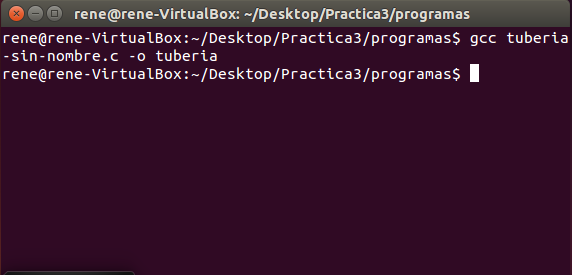
\includegraphics{imagenes/Captura.png}
		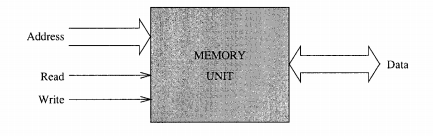
\includegraphics{imagenes/Captura2.png}
		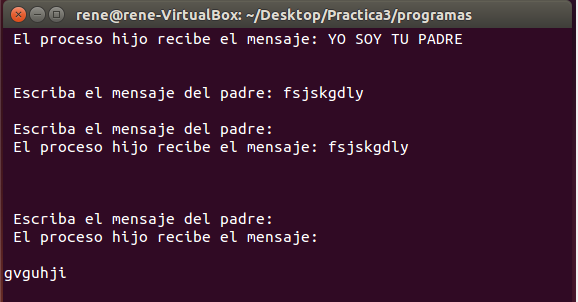
\includegraphics{imagenes/Captura3.png}
		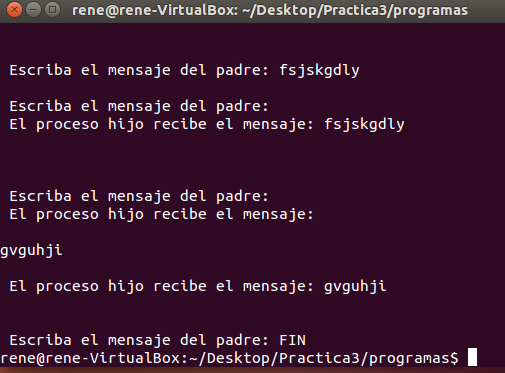
\includegraphics{imagenes/Captura4.png}
	\end{center}

	
	
	Para las siguientes funciones, mencione dónde están definidas, qué es lo que proporcionan de salida y qué argumentos necesitan de entrada:

	\begin{itemize}
		\item pipe 
		Esta funcion esta diseñada para interactuar entre los procesos padre e hijo, es una función unilateral donde uno solo puede escribir y el otro solo leer.
		Se necesita ingresar el array de la tuberia a interactuar.
		\item read
		 Read es una funcion que lee los valores ingresados por el usuario.
		Para poder  hacer uso de esta funcion es necesario ingresar el array donde se encuantra proceso padre,el array al que se hace referencia y el tamaño del array.
		\item write 
		Es una funcion en la que escribe en pantalla los valores ingresados en la funcion "fgets".
		Para hacer uso de esta funcion es necesario ingresar el array del proceso hijo, el mensaje previamente ingresado, y la longitud del mensaje a mostrar.
		*para este caso se le incremento en 1 al valor de la longitud del mensaje.
		\item fgets
		 Es una funcion que retorna  cadenas.
		Para poder hacer uso de la funcion fgets es necesario proporcionar El array donde se almacenara el mensaje, el tamaño del mensaje, asi como el tipo de entrada, ejemplo "stdin"=(Standard Input), es decir, por teclado.

	\end{itemize}
